\section{Introduction}

Cilia are microtubule-based hair-like projections of cells; in humans, they are found on nearly every cell of the body. Diseases known as ciliopathies where cilia function is disrupted can result in a wide spectrum of diseases. In primary ciliary dyskinesia (PCD), airway cilia that normally beat in synchrony to mediate mucus clearance can exhibit dyskinetic motion or become immotile, resulting in severe sinopulmonary disease\cite{o2007diagnosing}. Cilia defects have been associated with increased respiratory complications and poor postsurgical outcomes \cite{nakhleh2012high}. The characterization of ciliary motion abnormalities and specifics of the ciliary motion properties itself plays a critical role in the identification of specific ciliopathy and the determination of prophylactic respiratory therapies that could improve long-term outcomes in patients. Therefore, accurate identification of specific ciliary motion patterns is clinically compelling.

An objective, computational method for quantitative assessment of ciliary motion was proposed in~\cite{quinn2015automated}. In this work, ciliary motion was considered as an instance of dynamic texture \cite{saisan2001dynamic}. Dynamic textures are modeled as rhythmic motions of particles subjected to stochastic noise \cite{chen2013automatic}. Examples of dynamic textures include familiar motion patterns such as flickering flames, rippling water, and grass in the wind, each with a small amount of stochastic behavior altering an otherwise regular visual pattern. ciliary motion is well described as a dynamic texture. In [Quinn 2015], the authors found this representation robust for normal/abnormal binary ciliary motion classification, achieving an accuracy of over 90\% relative to expert ground-truth labeling.

While this study was instrumental in establishing the efficacy of dynamic textures as quantitative representations for ciliary motion, it was critically limited. First, the authors used autoregressive (AR) models \cite{hyndman2007higher} to model the dynamics of ciliary motion. While AR models are the preferred representation of dynamic textures, their primary use is in distinguishing between different types of dynamic textures, rather than between different instances of the same dynamic texture. Furthermore, the strong parametric assumptions imposed by the AR models on the underlying structure of the data -- multivariate Gaussian generating distributions that live on a linear manifold--severely restrict the representative power of AR models, truncating their sensitivity to minor but important variations in motion dynamics and rendering them incapable of capturing complex, nonlinear interactions.

Second, despite the considerable effort in automating much of the quantitative motion analysis, the authors still ultimately relied on expert clinician collaborators to manually select and extract regions of interest (ROI) from the raw video data to focus the analysis of the computational pipeline. These ROIs potentially introduce the same subjective bias of individual preference and training into the resulting data.

Here, we examine the application of deep learning, specifically convolutional neural networks (CNNs) to perform binary ciliary motion classification. CNNs do not impose strong parametric assumptions on the underlying data, instead capturing complex dynamics and interdependencies through a series of convolutional filters. Furthermore, CNNs do not require manual ROI selection in order to function, and can instead learn for themselves what feature maps to focus on.

3D convolutional neural networks provide a more scalable solution to ciliary motion classification while still incorporating information about the temporal structure inherent in video data of these cilia biopsies.

\section{Methods}

The objective of this experiment was to establish a baseline accuracy with a deep learning approach on cilia classification. To take advantage of the temporal dimension of video, a CNN with 3D convolution filters was implemented to classify ciliary motion. Similar computer vision techniques \cite{quinn2011novel} were used to preprocess the raw video data: specifically, derivatives of the optical flow were computed and differential flow invariants (rotation and deformation) were extracted and fed into the 3D CNN in batches

The dataset comprised of grayscale videos of nasal brush biopsies from 149 patients and examined by a blinded panel of clinicians. These videos were recorded at 200 frames per second for several seconds, and taken at 640x480 resolution. The panel of expert clinicians assigned labels to the patients to indicate degree of ciliary motion abnormality, where 1 constituted completely normal motion, 4 constituted highly abnormal motion, and 2 and 3 expressed gradations of abnormality. 

\begin{figure}[H]
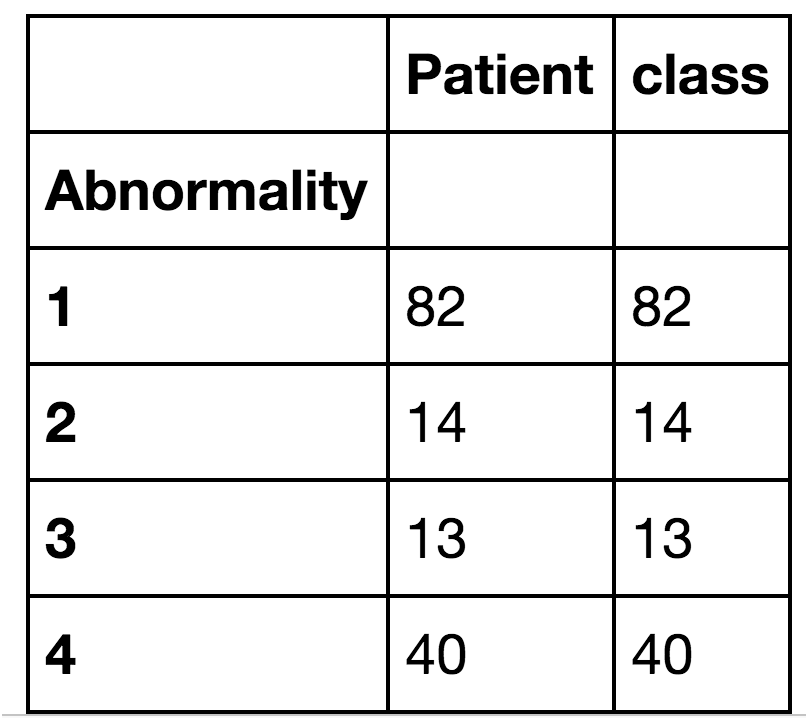
\includegraphics[scale=0.5]{patient_label}
\caption{A sample black and white graphic that has
been resized with the \texttt{includegraphics} command.}
\end{figure}

Multiple videos per patient were collected and each video was given the abnormality label of its patient. Some video samples were removed due to extraneous camera movement, poor lighting, bad focus, or other recording artifacts. Videos of patients with labels of 2 and 3 were removed from the training set, hopefully leaving more canonical examples of normal and abnormal motion for the network to learn from. This non-canonical subset of videos comprised 18.15\% of  the total 325 videos, leaving 266 videos left for training the network. Out of the canonical data, 127 videos or 47.77\% were labeled as examples of abnormal cilia motion, while the other half were labeled as normal.
 
Optical flow is used in computer vision to predict the probable motion of pixels between consecutive frames and represents movement of a pixel as a displacement vector field. Taking linear combinations of the derivatives of the optical flow yielded differential image invariants, colloquially known as measures of rotation, divergence, and deformation. These quantities are orientation-invariant, allowing ciliary motion to be analyzed irrespective of the camera orientation, lighting differences, or even the direction in which the cilia is beating~\cite{quinn2015automated}. The computed curl (rotation) of ciliary motion was used for training because it was the only component with scalar valued quantities. 
 
The videos were standardized to the absolute maximum value to preserve the most information when converting from floating point to 16 bit integer values. Some videos had extremely high maximum values so a scalar for each video was individually computed to prevent pixel value overflow and within range of data type. Each video had 250 frames, which were each reduced from $640 \times 480$ to $80 \times 60$ pixels and split into blocks of 10, effectively producing 25 arrays of $80 \times 60 \times 10$ inputs per video. These blocks were fed in batches of 10 per iteration into a 3D CNN implemented in Tensorflow and trained with a p2 instance on Amazon Web Services (AWS). 

\begin{figure*}
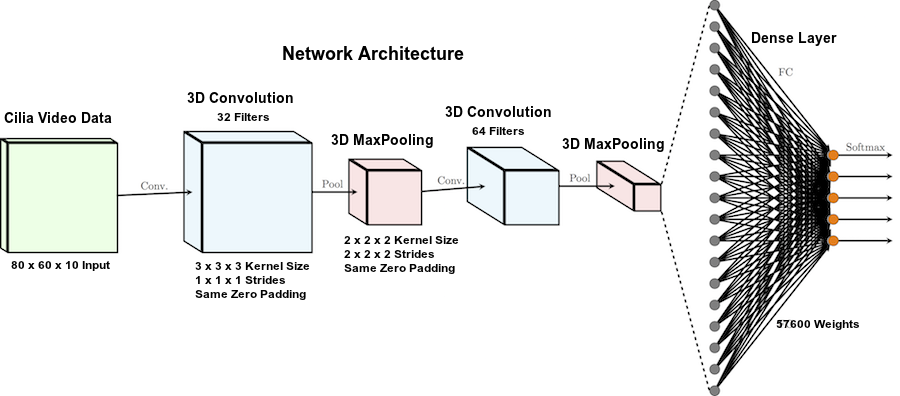
\includegraphics[scale=1.2]{arch}
\caption{Overview of the 3D CNN structure.}
\end{figure*}
%\setlength{\textfloatsep}{5pt}

\section{Results}

The 3D CNN architecture had 2 stacked layers, each composed of a 3D convolution layer and a 3D max pooling layer with Rectified-Linear Unit \cite{nair2010rectified} activation functions, and a fully connected layer outputting to a binary softmax classifier. Most CNN ``best'' practices \cite{goodfellow_bengio_courville_2016} were adapted for three dimensions. The first layer had 32 3D convolutional filters and the second layer had 64. The kernel size of each filter was $3 \times 3 \times 3$ and zero padding used and dropout \cite{srivastava2014dropout} added for regularization. The fully connected layer had 57600 weights due to $80 * 60 * 10 = 48,000$ plus 9,600 extra weights from zero padding. The varying learning rates were tried with ADAM~\cite{kingma2014adam} as the optimizer. A low batch size of 10 was selected to accommodate the memory capacities of our hardware resources. After 10 iterations, the model appeared to find a local minimum. We tested classification accuracy with a 66-33\% train-test split. 

The average performance of the 3D CNN on the test set was around 75\%, still below the 90\% the current state-of-the art benchmark from~\cite{quinn2015automated}. Using larger batch sizes and pixel dimensions slightly improved performance but made training much more computationally expensive and exhausted all memory capabilities of our machine. Trading dimension size of each frame for a larger block size had little difference in terms of accuracy but greatly increased computational memory requirements.  

\begin{figure}[H]
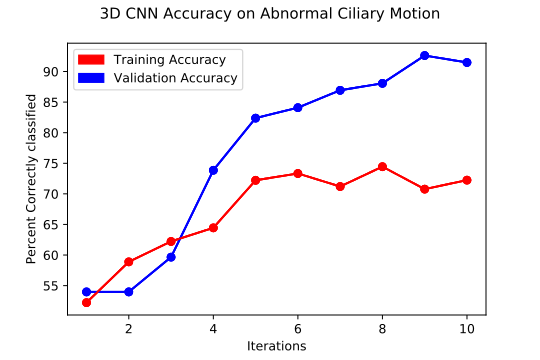
\includegraphics[scale=0.5]{CNN_graph}
\caption{Overview of the 3D CNN structure.}
%\setlength{\belowcaptionskip}{-10pt}

\end{figure}

We tested classification accuracy with a 66-33\% train-test split. The average performance of the 3D CNN of the test set is around 75\%, well below the 90\% benchmark of the current state-of-the art. 

\section{Discussion}

Clearly, the model is severely overfitting to the dataset. Several regularization techniques could be implemented to combat this: adding batch normalization, using data augmentation, and fine-tuning the weights. However, each pose their own difficulties. Most pre-trained network weights are designed for image input instead of video data and transfer learning \cite{pan2010survey} might be too generalized to differentiate the subtleties of ciliary motion. Data augmentation is feasible but must be done congruently with batches which would require more memory to be done online for video data. Also, the underlying structure of the rotation data might not allow for some of the same transformations as the raw grayscale videos of ciliary motion. Batch Normalization \cite{ioffe2015batch} would be rather straightforward to implement but would be unlikely to improve accuracy enough to current benchmarks. From experimenting with the dropout parameter, the 3D CNN model's learning capacity is too complex for its current input data. A better solution would be to provide the model with more labeled training examples and enough computing resources to allow for larger input dimensions. 
 
A limitation of this dataset was that each video was labeled at a patient level instead of per video, which might not contain any abnormal motion at all despite the patient being labeled abnormal or vise versa. We attempted to mitigate training on difficult and misleading examples by following~\cite{bengio2009curriculum} idea of curriculum learning by opting to only train on patients labeled 1 and 4, and this decreased the number of training examples.

Another limitation for the model was the drastic reduction in the dimensions of cilia data. The processed videos had to be reduced to 1/8 of their original size to avoid running into memory issues. This downsampling greatly diminished the network capacity to extract the most relevant features in distinct ciliary motion. With more computing resources and a more precisely labeled dataset, we would expect to see an increase in 3D CNN classification accuracy. With additional preprocessing, the deformation vector data could also be incorporated in addition to the rotation data to provide more relevant feature information for network to learn.

\section{Conclusion}

Although deep learning methods usually requires an abundant amount of labeled training data, one possible way to circumvent this issue would be to train a CNN to generate a heatmap of patches of the video where cilia are likely present, similar to the deep learning pipeline that won the Camelyon 17 challenge for Breast Cancer Classification~\cite{wang2016deep}. Then feed this into another classifier such as a Gradient Boosted Decision Tree or another CNN to predict abnormality of that cilia patch.
 
Other approaches that can leverage deep learning for cilia classification are Recurrent Neural Networks (RNNs) such as a Long-Short Term Memory (LSTM) network to actually incorporate a times-series element instead of simulating time with a third dimension in CNNs to build feature maps. It is even possible to stack CNNs on top of RNNs to get the best of both worlds. Others in computational have already applied this approach with good results \cite{sonderby2015convolutional}. Other rapidly growing areas of deep learning might be used to solve the broader problem of cilia segmentation and identification of ciliary motion phenotypes include attention-seeking mechanisms of RNNs and Reinforcement Learning in segmentation and  unsupervised deep learning techniques like General Adversarial Networks to generate a perfect canonical phenotype of ciliary motion.

%\end{document}  % This is where a 'short' article might terminate
